% !TEX TS-program = xelatex
% !BIB program = bibtex
% !TEX encoding = UTF-8 Unicode

\documentclass[
  twoside,
  openright,
  degree    = master,               % degree = master | doctor
  language  = english,              % language = chinese | english
  fontset   = template,             % fontset = default | template | system | overleaf
  watermark = true,                 % watermark = true | false
  doi       = true,                 % doi = true | false
]{ntuthesis}

\newcommand{\rustsec}{KrustVM}
\newcommand{\rustcore}{Rcore}
\definecolor{CodeGray}{RGB}{60, 60, 60}
\newcommand{\code}[1]{\texttt{\textcolor{CodeGray}{#1}}}

% !TeX root = ./main.tex

% --------------------------------------------------
% 資訊設定(Information Configs)
% --------------------------------------------------

\ntusetup{
  university*   = {National Taiwan University},
  university    = {國立臺灣大學},
  college       = {電機資訊學院},
  college*      = {College of Electrical Engineering and Computer Science},
  institute     = {資訊工程學系},
  institute*    = {Department of Computer Science and Information Engineering},
  title         = {實作基於Rust之安全Linux KVM虛擬機器監測器},
  title*        = {On Implementing a Secure Rust-based Linux KVM Hypervisor},
  author        = {章瑋麟},
  author*       = {Wei-Lin Chang},
  ID            = {R09922117},
  advisor       = {黎士瑋},
  advisor*      = {Shih-Wei Li},
  date          = {2023-07-11},         % 若註解掉,則預設為當天
  oral-date     = {2023-07-11},         % 若註解掉,則預設為當天
  DOI           = {10.6342/NTU202301822},
  keywords      = {系統安全, 虛擬化, KVM},
  keywords*     = {System Security, , Virtualization, KVM},
}

% --------------------------------------------------
% 加載套件(Include Packages)
% --------------------------------------------------

\usepackage[sort&compress]{natbib}      % 參考文獻
\usepackage{amsmath, amsthm, amssymb}   % 數學環境
\usepackage{ulem, CJKulem}              % 下劃線、雙下劃線與波浪紋效果
\usepackage{booktabs}                   % 改善表格設置
\usepackage{multirow}                   % 合併儲存格
\usepackage{diagbox}                    % 插入表格反斜線
\usepackage{array}                      % 調整表格高度
\usepackage{longtable}                  % 支援跨頁長表格
\usepackage{paralist}                   % 列表環境


\usepackage{lipsum}                     % 英文亂字
\usepackage{zhlipsum}                   % 中文亂字

% --------------------------------------------------
% 套件設定(Packages Settings)
% --------------------------------------------------


\begin{document}

% 封面與口試審定
% Cover and Verification Letter
\makecover                          % 論文封面(Cover)
\makeverification                   % 口試委員審定書(Verification Letter)

% 致謝與論文摘要
% Acknowledgement and Abstract
% !TeX root = ../main.tex

\begin{acknowledgement}

%首先,我要感謝我的指導教授黎士瑋博士,您帶領我走過一遍碩士班的研究過程,讓我受益良多。
%您在研究期間的建議不僅帶給我研究上的進展,其蘊含的分析角度也常比我自己的想法還更全面且有條理,讓我評斷一件事情的時候有更完整的思考。
%在撰寫論文的這幾個月,您不厭其煩的替我審閱我的論文,指出我文字描述中的邏輯謬誤和解釋不清之處,使得我的學術寫作及邏輯闡述能力更加精進。
%
%本論文的完成亦得感謝擔任我口試委員的黃敬群 (jserv) 教授與蕭旭君教授,因為你們的建議與意見,使得我的論文能夠更完整且嚴謹。
%
%另外感謝江昱勳與杜展廷同學,沒有你們的貢獻與合作,KrustVM的研究與投稿論文不會順利地完成。
%
%我也要感謝我的家人和朋友們,有你們的支持我才能完成論文。
%
%此外,特別感謝 OpenAI 的 ChatGPT,它不厭其煩的幫助我優化了論文的英文表達,許多論文中的字句 (包含了本致謝) 得益於它才能夠如此通順,清晰和流暢。
%
%最後,謹以此文獻給逝去的歲月。

首先,我要衷心感謝我的指導教授黎士瑋博士。在研究期間,您的指導和建議讓我受益匪淺。
您在研究期間的建議不僅帶給我研究上的進展,其蘊含的分析角度也常比我自己的想法還更全面且有條理,讓我學到評斷一件事情更完整的思考方式。
在撰寫論文的過程中,您不辭辛勞地審閱我的稿件,指出其中的邏輯謬誤和解釋不清之處,使我在學術寫作和邏輯闡述方面精進了許多。

本論文的完成亦得感謝擔任我口試委員的黃敬群 (jserv) 教授與蕭旭君教授,您們的寶貴意見和建議使得我的論文更加完整和嚴謹。
此外,感謝江昱勳與杜展廷同學的合作和貢獻,沒有你們的協助, KrustVM 的研究和論文投稿將不會如此順利地完成。
我也要衷心感謝我的家人和朋友們,是你們的支持讓我能夠順利完成論文。

特別感謝 OpenAI 的 ChatGPT,它不厭其煩地幫助我優化論文的英文表達。
許多論文中的文字,包括本致謝部分,都得益於它,使得我的論文變得更加通順、清晰和流暢。

最後,謹以此文獻給逝去的歲月。
\begin{flushright}
章瑋麟\\
%國立臺灣大學資訊工程學系暨研究所\\
中華民國一百一十二年七月
\end{flushright}

\end{acknowledgement}
       % 致謝(Acknowledgement)
% !TeX root = ../main.tex

\begin{abstract}

中文摘要

\end{abstract}

\begin{abstract*}

Commodity hypervisors play a vital role in cloud computing environments by
overseeing hardware resources for virtual machines. However, their growing
complexity and extensive attack surface pose significant security concerns.
An attacker that exploits vulnerabilities in the privileged hypervisor
codebase can gain unfettered access to VM data, compromising their safety.
Previous attempts to retrofit hypervisors into small trusted cores have
limitations, as the security still relies on the implementation of the trusted
core. Moreover, formal verification on the TCB necessitates significant human
effort and is not easily applicable to rapidly evolving codebases.
Recently, Rust adoption has been increasing for its strong memory safety
guarantees and performance efficiency.
This thesis addresses challenges in rewriting and porting the C-based KVM TCB
in SeKVM to Rust for a recent Linux long term support version. This allows the
resulting hypervisor, \rustsec{}, to not only benefit from recent Linux
advancements, but also be protected by Rust's safety guarantees.
Furthermore, the Rust-based implementation can be conveniently updated,
as Rust conducts safety checks at compile-time automatically.
%This thesis explores leveraging Rust to build a secure commodity hypervisor.
%We focus on rewriting SeKVM into KrustVM.
In \rustsec{}, a small trusted core written in Rust is incorporated to replace
the C-based core of SeKVM, which serves to protect VM confidentiality and
integrity.
%During the implementation of \rustsec{},
%we addressed challenges in linking a Rust TCB into Linux, rewriting SeKVM's
%C-based TCB in Rust, and bringing up \rustsec{} on real hardware.
%\rustsec{} incorporates
%\rustcore{}, a small trusted core written in Rust to protect VM confidentiality
%and integrity.
In addition,
a modular design is adopted to secure the trusted Rust core. We separated and
minimized the unsafe Rust code from safe Rust by enclosing unsafe code within
safe abstractions, and utilized Rust's type system to ensure the memory safety
of the unsafe memory accesses done by the trusted Rust core.
%[Then you focus on briefly disuss what you actually do -- enclosed unsafe code etc.]
%In addition,
%we minimized unsafe Rust usage, enclosed unsafe code within safe abstractions,
%and utilized Rust's type system to ensure the memory safety of unsafe
%operations in \rustcore{}.
\rustsec{} incurs modest overhead compared to mainline KVM and SeKVM, and
demonstrates the practicality of securing existing hypervisors through a
C-to-Rust rewrite.

\end{abstract*}
              % 摘要(Abstract)

% 生成目錄與符號列表
% Contents of Tables and Denotation
\maketableofcontents                % 目錄(Table of Contents)
\makelistoffigures                  % 圖目錄(List of Figures)
\makelistoftables                   % 表目錄(List of Tables)
% !TeX root = ../main.tex

\begin{denotation}[3cm]

\item[HPC]{
  高性能計算 (High Performance Computing)
}

\item[cluster]{
  集群
}

\item[Itanium]{
  安騰
}

\item[SMP]{
  對稱多處理
}

\item[API]{
  應用程序編程接口
}

\end{denotation}
            % 符號列表(Denotation)

% 論文內容
% Contents of Thesis
\mainmatter
\input{contents/chapter01}
\input{contents/chapter02}
\input{contents/chapter03}
\input{contents/chapter03}
\input{contents/chapter04}
\chapter{Evaluation}
\label{sec:eval}

We evaluated the performance of various application benchmarks
on a VM running on \rustsec{}, SeKVM, and mainline KVM.
We also tested the same
benchmarks on bare metal environment performances to establish a baseline
reference of the benchmark results. The workloads were run on the Raspberry
Pi 4 model B development board, with a Broadcom BCM2711, quad-core
Cortex-A72 (ARM v8) 64-bit SoC at 1.5GHz, 4GB of RAM, and a 1 GbE NIC device.

\rustsec{}, SeKVM, and the mainline KVM are all based on Linux 5.15.
QEMU v4.0.0 was used to start the virtual machines on Ubuntu 20.04. The guest
kernels also used Linux 5.15, and all kernels tested employed the same 
configuration. We requested the authors of~\cite{hypsec} and got a patch for
the Linux guest kernel to enable virtio.
\code{rustc} version 1.68.0-nightly was used to compile \rustcore{},
while clang 15.0.0 was used to compile the remaining components of
\rustsec{}, SeKVM, and the mainline KVM.
2 physical CPUs and 1 GB of RAM is configured for the bare
metal setup, and each VM is equipped with 2 virtual CPUs , and 1 GB of RAM.

We ran the benchmarks listed in \autoref{tab:benchmark} in VMs on
\rustsec{}, SeKVM, and the mainline KVM. \autoref{fig:eval} shows the normalized
results. In \autoref{fig:eval} we normalized the results to bare-metal
performance. 1.00 refers to no virtualization overhead, and
a higher value means higher overhead. The performance on real application
workloads show modest overhead overall for \rustsec{} compared to SeKVM and
mainline KVM. The overhead for \rustsec{} in most of the cases is less than
10\% compared to mainline KVM.
In the \code{TCP\_MAERTS} benchmark, all four experimental setups saturated the
1GbE NIC on the Raspberry Pi 4 model B. Additionally, experimental error had a
more noticeable impact during the measurement of the bare-metal setup, making
its performance the worst.
For \rustsec{}, \code{TCP\_RR} and the YCSB-Redis benchmarks experienced higher
overhead compared to mainline KVM at around 8\% and 14\%, respectively.
\code{TCP\_RR} and YCSB-Redis are benchmarks that both send a lot of small
packets, causing many VM exits. Hence, the bare-metal performance
is roughly twice as good as the VMs, amplifying the difference between mainline
KVM and \rustsec{} when plotting \autoref{fig:eval}.
%In fact, if the overhead are plotted by normalizing against the
%performance of mainline KVM (\autoref{fig:eval2}), all benchmarks run on
%\rustsec{} experience an overhead less than 10\% compared to mainline KVM.
In fact, when the overhead is normalized against the performance of the
mainline KVM (\autoref{fig:eval2}), all benchmarks executed on \rustsec{}
demonstrate an overhead of less than 10\% in comparison.
\rustsec{} performs nearly as well as mainline KVM in
CPU bound benchmarks and bulk data network performance benchmarks
(\code{TCP\_MAERTS}, \code{TCP\_STREAM}) since
the workloads require minimal to no VM exits.
The discrepancy arises in \code{TCP\_RR}, Apache, Memcached,
and YCSB-Redis, which involve a higher number of VM exits due to their frequent
small network transmissions. Both SeKVM and \rustsec{} execute additional logic
in EL2 to ensure VM data confidentiality and integrity, resulting in increased
overhead in VM exits compared to mainline KVM.
%The worst overhead for \rustsec{} compared to mainline KVM occurs for the
%YCSB-Redis benchmark at around 14\%.
%Various system noise factors e.g. caches, kernel thread wakeups, and dynamic
%voltage frequency scaling might also come into play.

\begin{table}
\centering
\footnotesize
\begin{tabular}{ |p{0.2\linewidth}|p{0.7\linewidth}| }
 \hline
 \small{\textbf{Name}} & \small{\textbf{Description}} \\
 \hline
 \small{Kernbench} & \small{Compilation of the Linux 6.0 kernel using \code{tinyconfig} for Arm with GCC 9.4.0.} \\
 \hline
 \small{Hackbench} & \small{\code{hackbench}~\cite{hackbench} using Unix domain sockets and 50 process groups running in 50 loops.} \\
 \hline
 \small{Netperf} & \small{\code{netperf}~\cite{netperf} v2.6.0 running the netserver on the server and the client with its default parameters in three modes: TCP\_STREAM (throughput), TCP\_MAERTS (throughput), and TCP\_RR (latency).} \\
 \hline
 \small{Apache} & \small{\code{Apache} v2.4.41 Web server running \code{ApacheBench}~\cite{ab} v2.3 on the remote client, which measures the number of handled requests per second when serving the 41 KB index.html file of the GCC 4.4 manual using 100 concurrent requests.} \\
 \hline
 \small{Memcached} & \small{\code{memcached} v1.5.22 using the \code{memtier}~\cite{memtier} benchmark v1.2.3 with its default parameters.} \\
 \hline
 \small{YCSB-Redis} & \small{\code{redis} v7.0.11 using the \code{YCSB}~\cite{YCSB, YCSB2} benchmark v0.17.0 with its default parameters.} \\
 \hline
\end{tabular}
\vspace{0.3cm}
\caption{Application Benchmarks}
\label{tab:benchmark}
\end{table}

\begin{figure}[hbtp]
    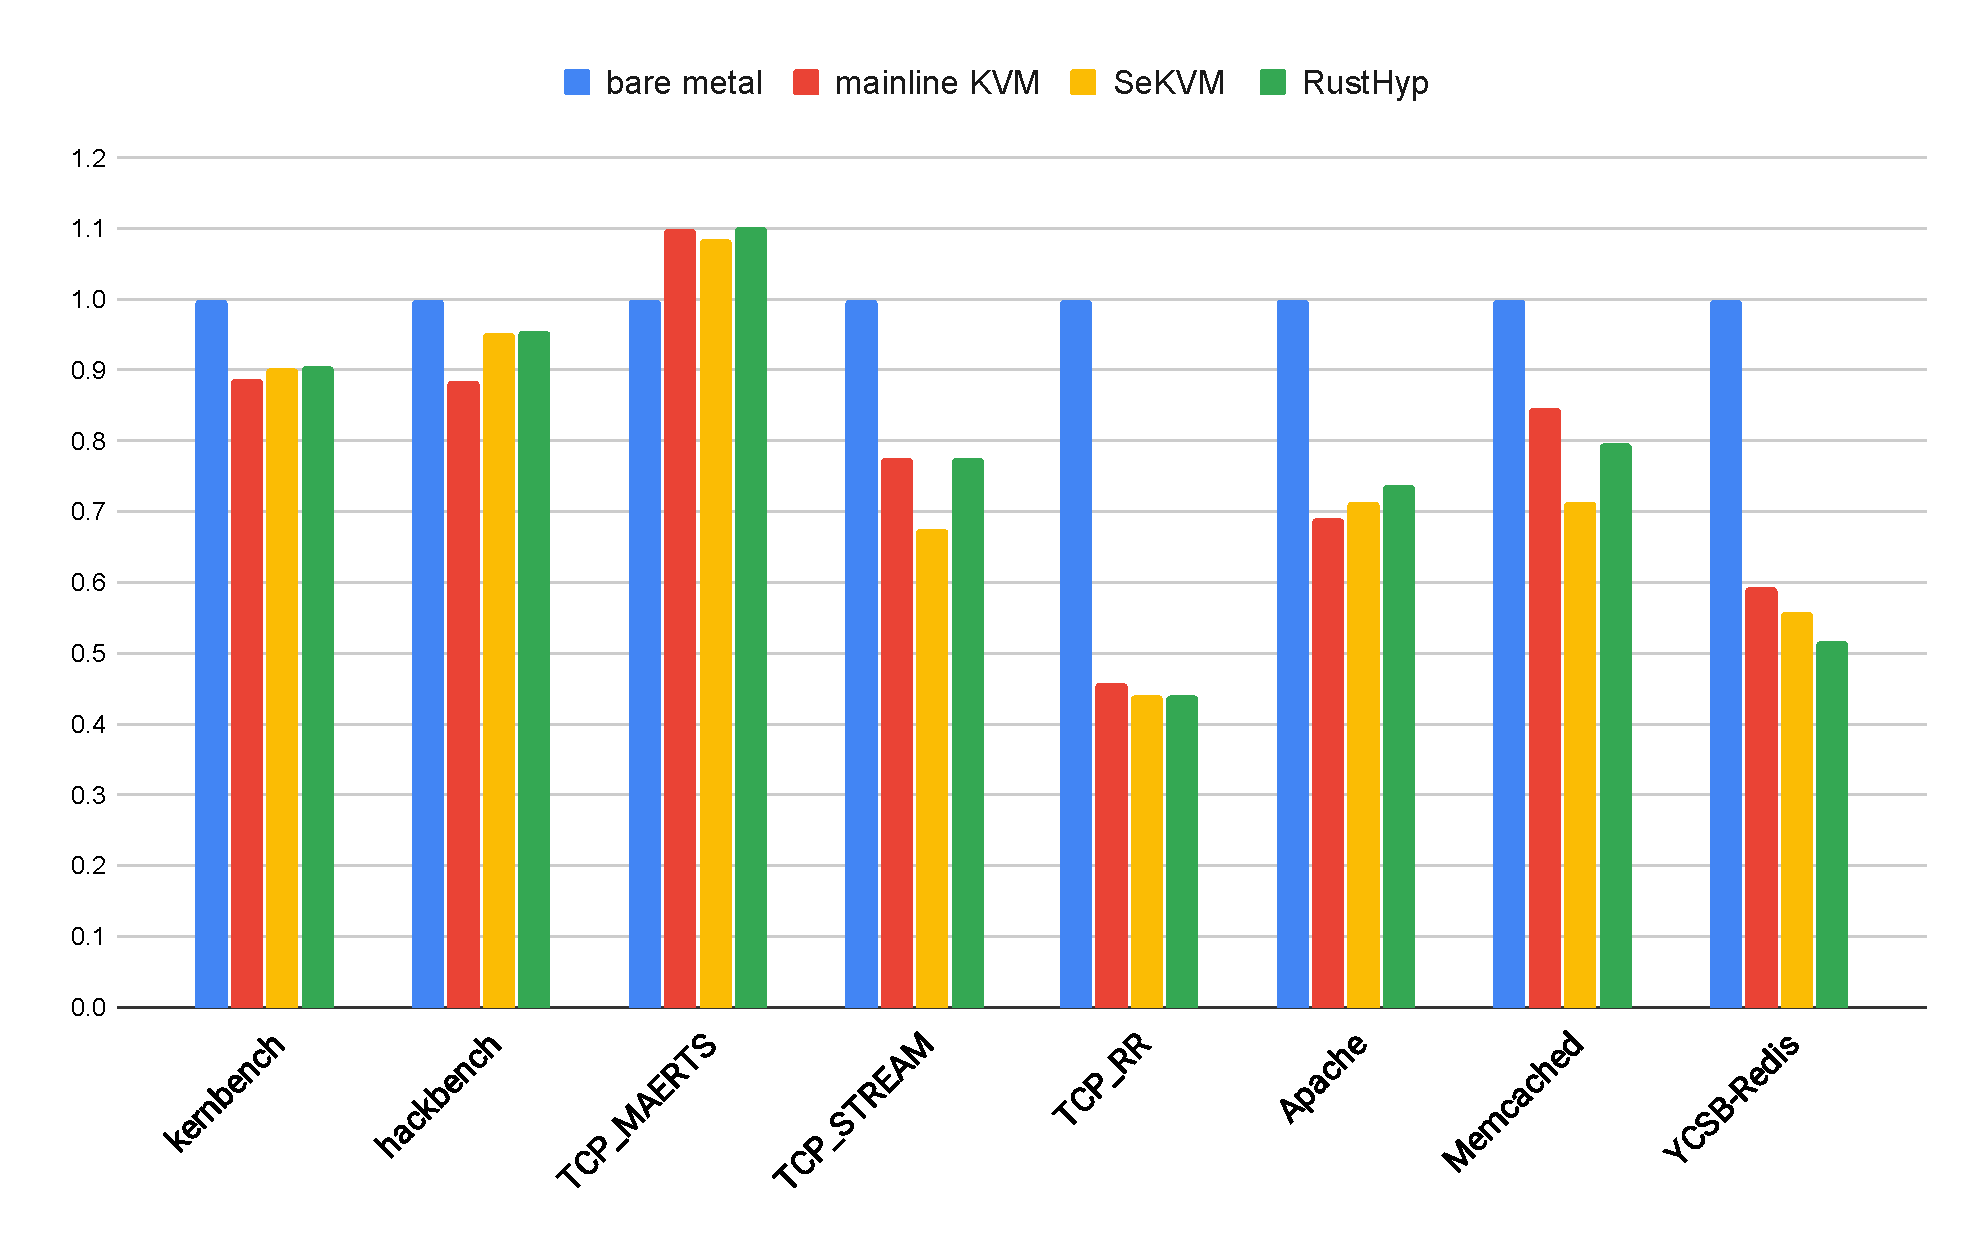
\includegraphics[scale=0.45]{figures/eval.pdf}
    \caption{Application Benchmark Performance: Overhead normalized to the bare-metal setup}
    \label{fig:eval}
\end{figure}

\begin{figure}[hbtp]
    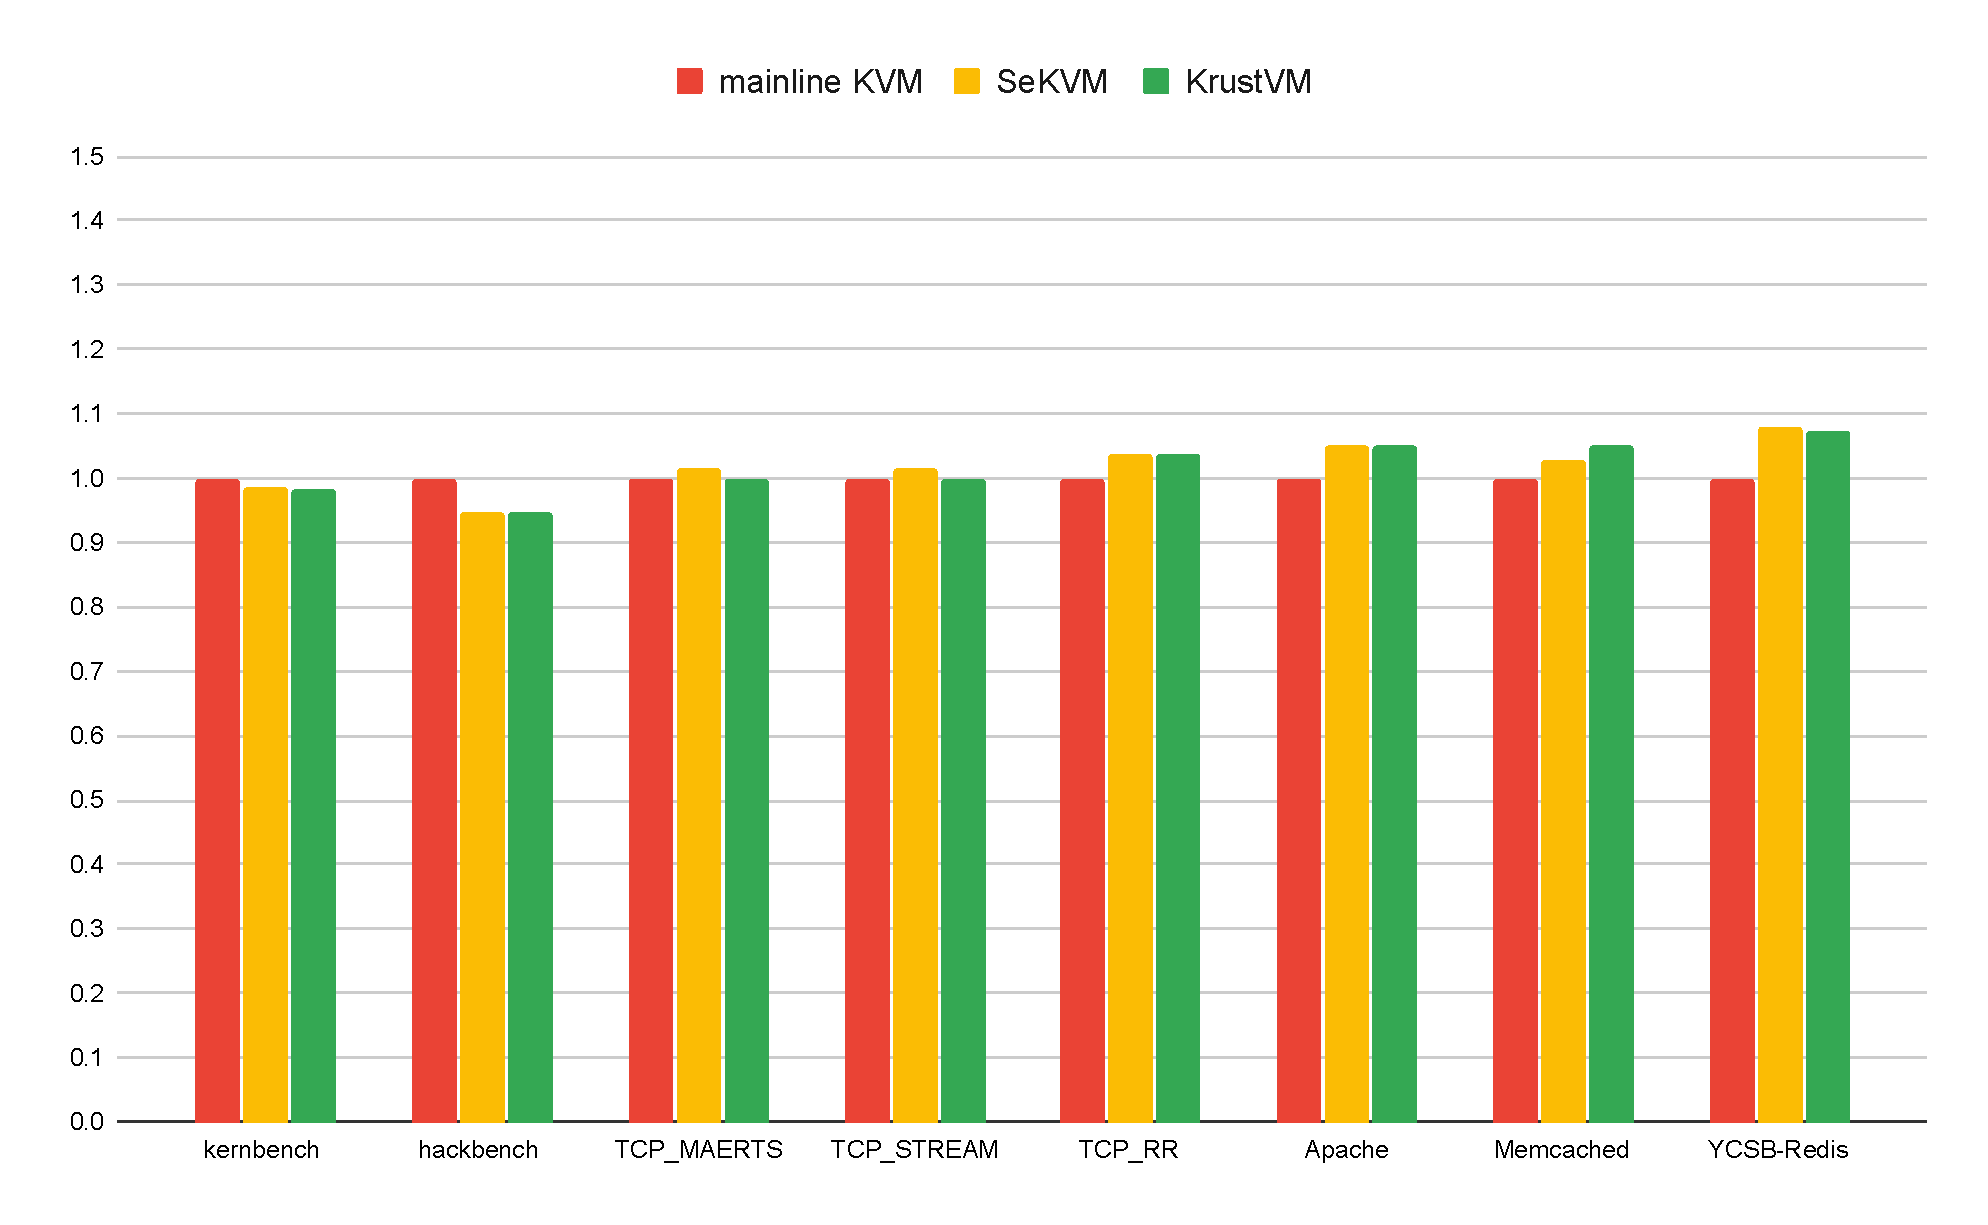
\includegraphics[scale=0.45]{figures/eval2.pdf}
    \caption{Application Benchmark Performance: Overhead normalized to mainline KVM}
    \label{fig:eval2}
\end{figure}


% 參考文獻
% References
\refmatter
\bibliographystyle{abbrv}
\bibliography{back/references}

% 附錄
% Appendices
\input{back/appendix01}
\input{back/appendix02}

\end{document}
